\clearpage
\subsection{Summary} % (fold)
\label{sub:arrays_summary}

This Chapter introduced a number of concepts related to working with multiple values in code.

\begin{figure}[h]
   \centering
   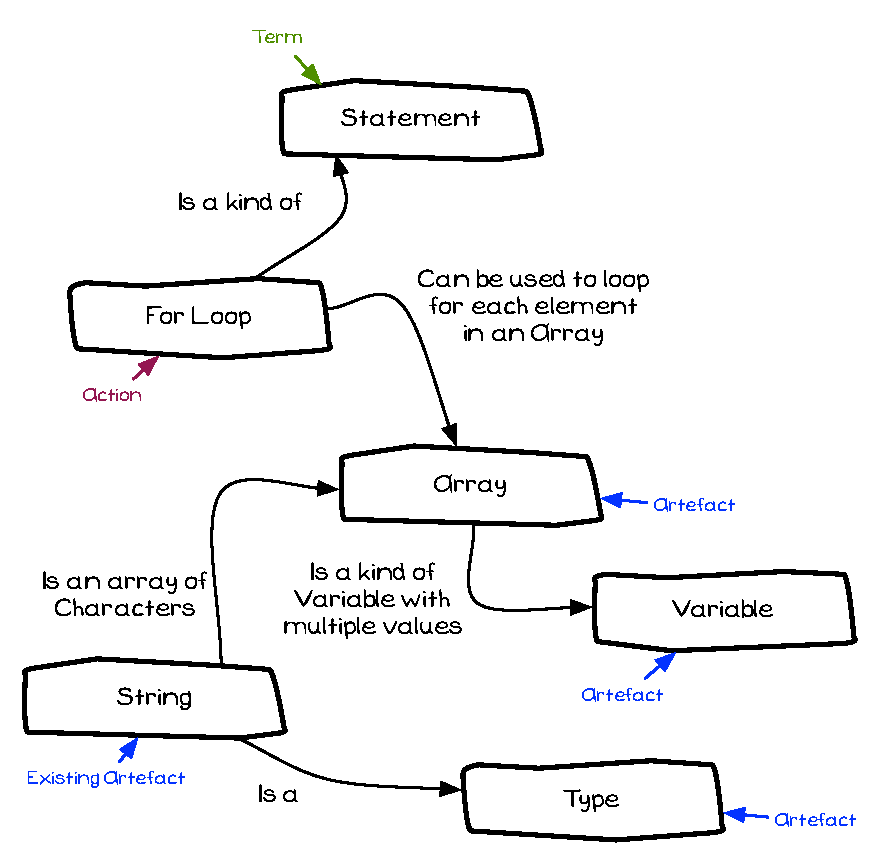
\includegraphics[width=0.8\textwidth]{./topics/arrays/diagrams/Summary} 
   \caption{Concepts covered in this Chapter}
   \label{fig:arrays-summary}
\end{figure}

\mynote{
\begin{itemize}
  \item The central concept of this chapter is the \nameref{sub:array}. An array is a variable that can store multiple values.
  \item When you work with arrays make any logic you want to apply to \emph{all elements} will be coded using \textbf{for each} element and the \nameref{sub:for_loop}.
  \item \nameref{sub:string}s are arrays of characters, and can be used to store textual data in your code.
\end{itemize}
}


% subsection summary (end)
